\section{Overview of the Approach}

In the current thesis, we propose a client-based approach for the integration
open-source productivity software to enterprise document management systems. So
we discuss the case here when an enterprise company tries to replace the client
part of the document management system with an open-source alternative, while
keeping the existing proprietary server-side part of the system. As a
consequence, the center of my approach is the client -- the document management
part of the client, to be more exact (figure~\ref{fig:overview-architecture}).

\begin{figure}[H]
\centering
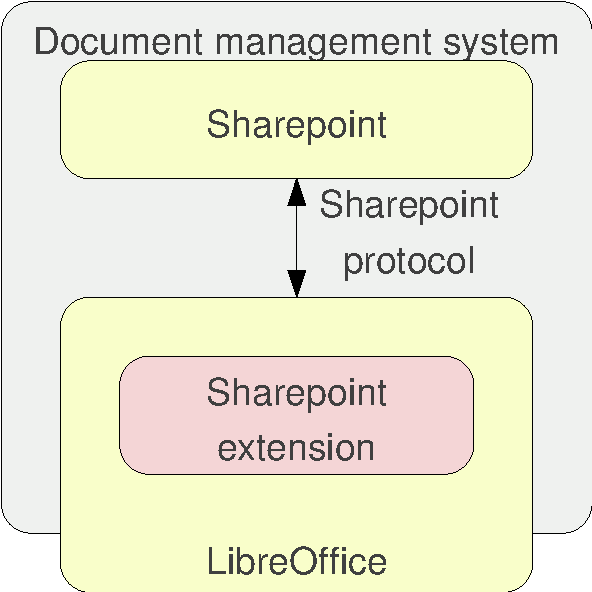
\includegraphics[width=250px,keepaspectratio]{overview-architecture.pdf}
\caption{Architecture of the approach}
\label{fig:overview-architecture}
\end{figure}

Components of the above example can be replaced, for example the Alfresco (with
its SharePoint module) can be used in place of SharePoint, and OpenOffice.org
can be used in place of LibreOffice. The SharePoint server, the office
productivity suite is already present.

By observing the network traffic between the SharePoint server and a native
Microsoft Office, the protocol can also be known. As mentioned earlier, the
documentation on its own is not enough, as it's not complete\footnote{And it's
purely a reference, there are no guide or tutorial to get started.}.

Finally at this stage the only remaining component is the SharePoint extension
in LibreOffice what is missing, and my approach creates that.

Note that Alfresco already has an OpenOffice.org extension called
OPAL\cite{opal}. That naturally uses Alfresco's native protocol to communicate
with the server. The following major changes are needed to make to suit our
needs:

\begin{itemize}
\item It's intended to be used with OpenOffice.org 3.1 -- the last stable
version of OpenOffice.org is 3.3, and it won't work with this version. The
oldest stable release of LibreOffice is based on OpenOffice.org 3.3 as well, so
poring the extension to 3.3 is essential to make it working at all with
LibreOffice.
\item It works by installing an additional module on the Alfresco server, so
the business logic is minimal in the extension. My approach is to communicate
without any server-side component installations required.
\item The SharePoint protocol supports more than Alfresco, the user interface
has to be extended to cover the new features.
\item Finally the used protocol has to be changed: by using the SharePoint
protocol, the extension can communicate with both SharePoint and Alfresco,
covering a lot from today's enterprise document management server
installations.
\end{itemize}

Now that we understood what component we want to create and from where, it's
essential to see what workflow the document management clients take part in:

\begin{figure}[H]
\centering
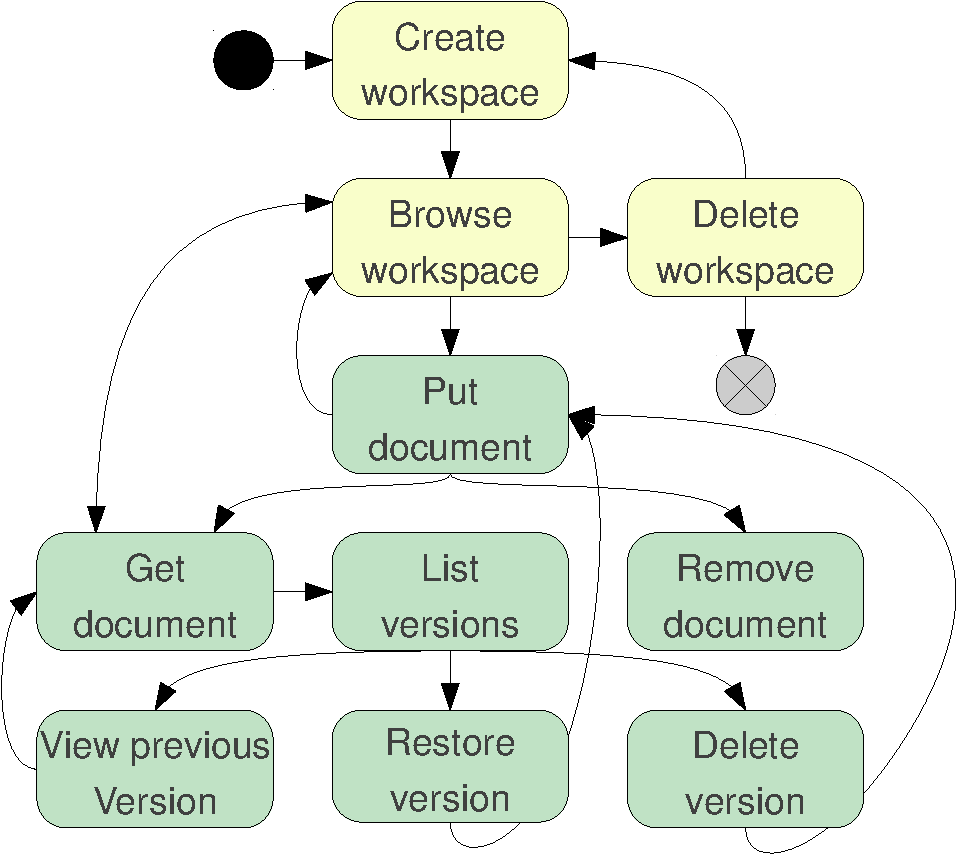
\includegraphics[width=300px,keepaspectratio]{overview-workflow.pdf}
\caption{Workflow of the approach}
\end{figure}

The workflow has the following steps:

\begin{itemize}
\item Create workspace: It creates a document workspace, which is the top-level
container for any document stored on the document management server.
\item Browse workspace: An existing workspace can be browsed, and a documents
can be put to workspaces.
\item Delete workspace: It's possible to get rid of no longer needed workspaces.
\item Put document: After selecting a target folder (using browse), a document
can be uploaded.
\item Get document: Existing documents can be downloaded for viewing or editing.
\item Remove document: Unneeded documents can be removed individually.
\item List versions: Every upload of a document may (depending on its type)
create a new version of the document. We can retrieve the list of this change log.
\item View previous version: older instances of a document can be viewed
read-only anytime.
\item Restore version: it's possible to revert all changes after a given
version with this step.
\item Delete version: older versions can be deleted.
\end{itemize}

In this section, I shown what component of the document management system I
plan to implement. The next section will describe how the implementation is
designed to happen.
